\documentclass[12pt]{article}
\usepackage{graphicx}
\usepackage{fullpage}
\input{epsf}


% Direct setting of margins:
% \addtolength{\oddsidemargin}{-0.875in}
% \addtolength{\evensidemargin}{-0.875in}
% \addtolength{\textwidth}{1.75in}
%
% \addtolength{\topmargin}{-0.875in}
% \addtolength{\textheight}{1.75in}

%\twocolumn
\raggedright
\setlength{\parindent}{0.2in}


\title{Rendering Massive Terrains using Chunked Level of Detail Control\\DRAFT}
\author{
        Thatcher Ulrich\\
        Oddworld Inhabitants\\
        tu@tulrich.com\\
}
\date{Revised 14 April 2002}

\begin{document}

\maketitle


\begin{figure}[h]
\centering
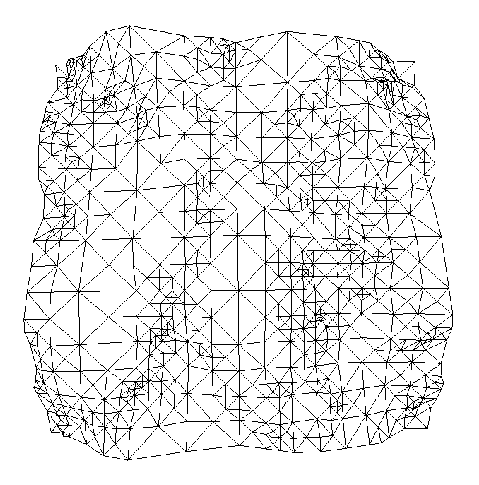
\includegraphics[height=2.1in]{sig-fig-tree1}
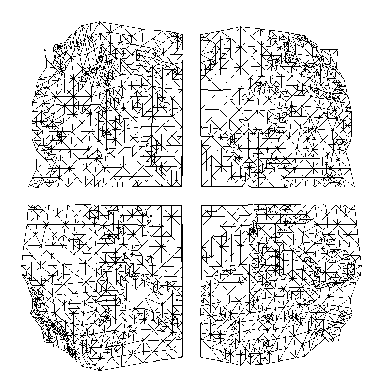
\includegraphics[height=2.1in]{sig-fig-tree2}
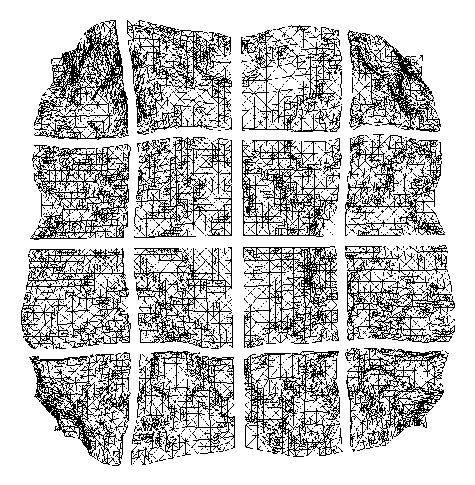
\includegraphics[height=2.1in]{sig-fig-tree3}
\caption{The first three levels of a Chunked LOD tree.}
\label{fig:tree}
\end{figure}


\section{Introduction}

Outdoor terrain rendering is important for a large class of game and
simulation applications.  Hardware and algorithms continue to improve
rapidly, which enhances our ability to render realistic terrains.  The
shift in recent years in consumer hardware from CPU bound graphics
pipelines to high speed special purpose graphics processing units
(GPUs) has drastically changed the tradeoffs in geometric level of
detail (LOD) terrain rendering algorithms.  These new tradeoffs have
sparked the development of GPU-oriented {\em aggregated } LOD
algorithms.  Furthermore, the increased quantity and detail of the
data sets we can render has raised the demand for data to feed to our
renderers, and highlighted the importance of handling data sets which
do not fit in RAM ({\em out-of-core } data sets).  Meanwhile, advances
in shading and image quality in general have raised end-users'
expectations for image quality and lowered their tolerance for visual
artifacts.
 
These notes briefly review the problems of constructing an ideal
terrain renderer, mention the most popular and successful existing
algorithms, and then present Chunked LOD, a novel approach to
aggregated LOD.  Chunked LOD has a number of practical advantages over
previous schemes, including ease of texturing, low CPU load and simple
handling of out-of-core data sets.
 
\section{The Ideal Terrain Renderer}

The ideal terrain renderer would let the viewer stand at the summit of
a tall mountain and see the surrounding countryside in perfect detail,
from the trees on a distant ridge line to the pebbles at the
viewer's feet.  The viewer would freely move around the scene,
walking through dense forests or flying rapidly through the air
directly to some distant spot, where both the local surroundings and
distant vistas would always be perfectly detailed to within the limits
of the display.  The place represented by the ideal terrain renderer
could be a faithful model of part of the real world, or some imaginary
locale, but in either case should be visually rich and interesting.
At no point should the viewer be aware of any distracting artifacts
arising from the shuffling of data or reorganizing of geometry within
the renderer itself.
 
Unfortunately we are not yet able to make the ideal terrain renderer.
In the meantime we would like to get as close as we can with the
technology we do have, and it turns out that we can do quite well in
some respects.
 
\section{Heightfields and LOD}

In these notes I am going to restrict my focus to heightfield
rendering.  Heightfield rendering is a smaller, but important,
sub problem of constructing the ideal terrain renderer described above.
Heightfields are not strictly necessary, and in fact are not
sufficient in themselves for ideal terrain rendering, especially when
the viewer gets close to the ground.  But the heightfield format is a
very useful approximation.  It embodies a basic method of compression
and a framework for organizing data and textures.  There are also many
existing heightfield algorithms, tools and data sets to build on.

% extension to general meshes
 
There are a number of good solutions for heightfield level of detail
(LOD) rendering which effectively reduce the number of triangles which
need to be rendered, at the expense of doing some run-time meshing
calculations.  Probably the most popular approach is to use a
restricted quadtree or binary-triangle tree.  The most commonly cited
papers are \cite{lindstrom96}, \cite{duchaineau} and \cite{rottger},
and they all work quite well, with a number of publicly available
implementations.  They generally involve some preprocessing and a
little extra per-vertex error data over and above a standard
heightfield.  Another important set of LOD algorithms is derived from
Hoppe's Progressive Meshes \cite{hoppe96}.  PMs focus on general meshes rather
than heightfields in particular, which results in somewhat different
trade offs, but have been successfully applied to heightfields.
 
\section{Detail and visual richness}

A major problem that soon becomes apparent when you experiment with
demos of these systems is the limited amount of detail present in the
data.  The frame rate is high, the mesh is seamless, but when you get
close to the ground things get very blurry and smoothed out, and when
you go high into the air you eventually see the edge of the data.

The difficulty here is that we just cannot store enough heightfield
and texture data in RAM to get the detail we want over large areas.
One typical solution is to store a very large data set out-of-core ---
on a local disk, or on a networked server --- and page in only the
data required for a particular view.  Several of the LOD references,
particularly \cite{lindstrom01}, address the issue of out-of-core
storage, but high quality consumer-level solutions are still lacking. % ``ad-hoc''?

From a game programming perspective, there are also some alternative
approaches to making huge terrains that do not involve out-of-core
storage at all.  One approach is to use adaptive detail, using a
multiresolution representation so that `important' areas of the
terrain have lots of data, while less important areas use very little
data.  This can nicely solve some practical problems, but is not a
general solution, as it puts detail and richness in the virtual world
in conflict with freedom of movement for the viewer.

Another approach is to create procedural detail on the fly as it is
needed.  This is a very powerful technique, but has significant
limitations.  The difficulties here include processing time ---
beautiful and interesting terrains can be generated procedurally with
packages like Bryce or Mojoworld, but achieving such high quality
takes a lot of processing time, and must typically be done in a
preprocessing stage.  Another open problem is making procedural
terrains controllable enough so that game designers and artists can
achieve the specific results they want.

% Compression is closely related to procedural detail, and can help
% bridge the gap ...

% instancing
 
In these notes I am focusing mainly on rendering large, static
out-of-core data sets, since the trade-offs are less
application-dependent than with procedural or adaptive detail.
Nevertheless, I don't want to minimize the importance of these other
approaches.  Real applications usually need to implement some
combination of approaches to achieve good results.
 
\section{Level of Detail and Perspective}

Because of perspective, when we stand on a terrain in the real world
and look out over a vista, our view covers a wide scale of geometric
detail.  We can resolve 1mm details in the pebbles at our feet, but in
the far distance, a 100m cliff on the side of a mountain may be the
smallest thing we can resolve.  That is a factor $10^5$ in geometric
size difference, due entirely to perspective.  Exploiting this effect
is central to scalable terrain LOD control.
 
The good existing schemes generally can guarantee that a mesh is
rendered within some maximum screen-space error tolerance,
$\tau$, while taking advantage of the perspective transform
to render fewer and fewer triangles as distance from the viewer
increases.
 
\section{Texturing}

Texture mapping sometimes gets short shrift in the terrain LOD
literature, but in practice it is critical for good visual results.
Shading is a key indicator of geometric shape and detail, but it is
impractical to achieve quality pixel-level fine detail using geometry
only.  Among other things, graphics hardware is much better at
antialiasing minified textures than it is at antialiasing sub-pixel
vertex shading.  Textures are also relatively compact for this
purpose.
 
Like our geometry, we would like our texture mapping to be scalable
over a $10^5$ range of detail levels.  Fortunately, it is not as
difficult to seamlessly match up texture edges as it is to match up
geometry edges.  Quadtree tiling is a straightforward, fully scalable
solution to the problem \cite{ulrich01}.  A serious difficulty lies in
integrating tiled texturing with scalable geometric LOD.  We cannot
draw more than one texture map per triangle, and for efficiency we
would like to draw many triangles with the same texture.  At the same
time, for image quality and to avoid LOD artifacts, we would like to
maintain a texture density of least one texel per visible pixel on
screen.  We need our geometric LOD solution to be compatible with
those constraints.
 
\section{Pre-GPU LOD Algorithms}

In these notes, I am using the term GPU to refer to a class of low
cost high speed specialized vertex processing hardware, such as the
NVIDIA GeForce, ATI Radeon and Sony PlayStation 2.  This class of
hardware incorporates one or more floating point transformation units
in addition to the integer pixel rasterization hardware common in the
previous generation of consumer graphics hardware.  The floating point
vertex processing done by these high speed GPUs had previously been
the responsibility of the general purpose CPU, greatly limiting
triangle throughput.
 
Prior to the widespread adoption of GPUs, LOD algorithms for game
applications focused on minimizing the number of triangles drawn, at
the expense of a limited amount of extra CPU processing.  Various
published algorithms for this, such as Lindstrom-Koller CLOD
\cite{lindstrom96}, ROAM \cite{duchaineau} and Progressive Meshes
\cite{hoppe96} were adopted and adapted to become a useful component
in the game programmer's toolbox.  The additional processing necessary
to compute scalable LOD meshes was typically more than made up for by
the time saved by transforming fewer vertices for rendering.

\section{Post-GPU LOD Algorithms}

With the advent of GPUs, consumer hardware saw maximum triangle
rendering rates skyrocket.  CPU involvement in rendering could be
limited to merely pointing the GPU at a section memory containing the
vertices of a model to render.  Developers interested in producing top
quality graphics for games often focus on either brute force all-GPU
methods (i.e. no continuous LOD), or approaches with very low CPU
overhead, like View Independent Progressive Meshes
\cite{bloom}\cite{svarovsky}.
 
Unfortunately, those algorithms are not view dependent, and it is not
obvious how to scale these methods to terrain data sets with a
seamless $10^5$ ratio between near and far detail.  Likewise,
reorganizing the continuous LOD approaches to achieve low CPU overhead
presents many difficulties.
 
\section{Chunked LOD}

Nevertheless, an efficient, hardware-friendly continuous LOD algorithm
is highly desirable, and there are a number of published approaches
that have achieved success at solving the core geometric LOD problem.
These approaches commonly exploit two strategies individually or in
combination:
 
\begin{enumerate}
\item Apply a view-dependent LOD algorithm to aggregates of
primitives, not individual primitives.

\item Cache the results of a vertex-level LOD algorithm to reuse them
for similar viewpoints.
\end{enumerate}

Various approaches are detailed in \cite{deboer}, \cite{bloom},
\cite{cline}, \cite{levenberg} and \cite{pomeranz}.  The permutations
are too numerous to summarize here, so I refer you to the individual
descriptions.
 
Chunked LOD is yet another variation on strategy 1 above.  Like some
of the other aggregated approaches, it achieves low CPU overhead and
high triangle throughput.  However, it uniquely combines several
other important advantages:

\begin{itemize}

\item Efficient use of triangles within aggregates.

\item Texture LOD integrated with geometry LOD.

\item Easy to integrate with out-of-core storage.

\item Efficient, smooth vertex morphing; no vertex pops.

\item Low CPU load, even when viewpoint moves rapidly.

\end{itemize}

The negative characteristics include:

\begin{itemize}

\item Non-trivial preprocessing required.

\item Data set must be static.

\item Uses more triangles than a primitive-level algorithm, for the same
  screen-space error.

\item Some data size overhead, depending on lossiness of preprocessing.

\end{itemize}

The general approach to Chunked LOD is laid out in \cite{bloom},
although in the context of using view-independent progressive meshes
for the chunks.  \cite{cline} covers the usage of quadtrees of meshes,
with morphing of static meshes to avoid popping artifacts, but relies
on regular grid subdivision within each mesh, and is not easily
amenable to out-of-core paging.

The method presented in these notes builds on those ideas and works
out a number of important details.
 
At the heart of the method is a tree of static, largely independent
preprocessed meshes.  The tree and its component meshes (the
``chunks'') are generated in a preprocessing step, based on a
high-detail reference mesh.  Each chunk is just a static mesh
primitive that can be rendered with a single glDrawElements() or
DrawPrimitive() call, plus an additional fast morphing pass.  The
chunk at the root of the tree is a low-detail representation of the
entire object.  The child chunks of the root node split the object
into several pieces, and each piece independently represents its
portion of the object with a higher level of detail than the parent.
 
This relationship is recursive down to some arbitrary depth.  Each
chunk has a bounding volume associated with it, as well as a maximum
geometric error, $\delta$.  $\delta$ represents the maximum geometric
deviation of a chunk (in object space) from the portion of the
underlying full-detail mesh it represents.
 
For simplicity's sake, I assign the same $\delta$ to all the meshes at a
particular level in the chunk tree.  Furthermore, I compute $\delta$ such
that:

\begin{equation}
\delta(L + 1) = \frac{ \delta(L) }{ 2 }
\label{eq1}
\end{equation}

Where $L$ is the level in the tree.  For example, if the root node of
the tree is a single mesh that represents the object with at most 16
units of deviation from the original full-detail mesh ($\delta(0) = 16$)
then the second level contains several chunks that each represent a
piece of the object with at most 8 units of deviation from the
full-detail mesh ($\delta(1) = 8$).  At the fifth level down the tree, the
chunks each represent a small piece of the object, with only 1 unit of
deviation ($\delta(4) = 1$).
 
When we apply this splitting scheme to a heightfield, the simplest
approach is to organize the tree as a quadtree of heightfield
sub-squares (see figure \ref{fig:tree}).  This will also prove
convenient when we consider texture mapping.
 
\section{View dependent rendering}

At run time, to render the object, we simply choose the chunks that
represent each part of the object to meet our desired visual fidelity.
Since we have a bounding volume for each chunk, and a maximum
geometric error for the vertices within a chunk, we can use a standard
LOD formula for conservatively determining the maximum screen-space
vertex error, $\rho$, for a chunk:

\begin{equation}
\rho = \frac{ \delta }{ D } K
\label{eq2}
\end{equation}
 
Where $\delta$ is the maximum geometric error of a chunk, $D$ is the
distance from the viewpoint to the closest point on the chunk's
bounding volume, and $K$ is a perspective scaling factor that takes
into account the viewport size and field-of-view, and is computed by:
 
\begin{equation}
K = \frac{ viewportwidth }{ 2 \tan \frac{horizontalfov}{2} }
\label{eq3}
\end{equation}
 
Note that, as is common in the LOD literature, $\rho$ is measured at
the center of the viewport, which is slightly liberal but reasonable.
From the standpoint of efficiency, there is no compelling reason not
to use a more precise, more expensive screen-space error metric;
unlike per-vertex LOD algorithms, the view metric typically only needs
to be evaluated on the order of a couple hundred times per frame.
Nevertheless, this simplified metric is very effective in practice,
and because it is independent of view direction, the LOD mesh stays
absolutely stable when the viewer rotates in place.
 
A simple way to evaluate our LOD tree and render the chunked model is
to traverse the tree, starting at the root.  We start out by choosing
a value for our maximum tolerable screen-space error, $\tau$.
Then, given a chunk, we can use equation \ref{eq1} to determine whether the
screen-space error is acceptable.  If it is, then we render the chunk
and do not recurse to the children.  If it is not acceptable, then we
recurse to the child nodes.  Pseudocode:

% \begin{verbatim}

\begin{ttfamily}
\begin{tabbing}
\hspace{0.25in}\=\hspace{0.25in}\=\hspace{0.25in}\=\hspace{0.25in}\=\hspace{0.25in}\= \\
function render\_lod(node)                                                      \\
\>      if rho(node, viewpoint) $<=$ tau then                   \\
\>\>            draw(node.mesh)                                                 \\
\>      else                                                                    \\
\>\>            for c in node.children do                                       \\
\>\>\>                  render\_lod(c)                                          \\
\>\>            end                                                             \\
\>      end                                                                     \\
end                                                                             \\
\end{tabbing}
\end{ttfamily}

% \end{verbatim}

There are two big problems with the above algorithm:
 
\begin{enumerate}

\item Neighboring chunks at different LODs will have cracks where they meet.

\item When the viewpoint approaches a chunk, the chunk will split into
several child chunks, and the mesh shape will pop suddenly.  Because
many vertices are popping at the same time, this is much more
objectionable than the single vertex popping in common ROAM or
PM-based implementations.

\end{enumerate}

Effective solutions to both problems follow.
 
\section{Crack filling}

There are several ways to fix the cracks between meshes.  One obvious
approach is to always decimate the edges of chunks to some globally
constant geometric error, regardless of the chunk's actual $\delta$.
Unfortunately this severely limits scalability.  A better variation on
this is to restrict the relationship of neighboring chunks, and always
decimate to a regular scale-relative pattern at the edge
\cite{levenberg}\cite{pomeranz}, although this is not optimal either.
 
\begin{figure}[h]
\centering
\includegraphics[width=6in]{sig-fig-flange}
\caption{Using a flange to fill a crack.  The white triangle on the
left is a crack between two meshes.  A flange (marked in black) is
added to one of the meshes; it extends into the other mesh and
inter-penetrates, covering the crack.}
\label{fig:flange}
\end{figure}

Another method is to add `flanges' around each chunk, so the meshes
interpenetrate slightly.  This should usually work well, but avoiding
artifacts gets a little messy.  In particular, choosing the angle and
size of the flanges is somewhat ad hoc and depends on the precise
geometry of the neighbor.  Proper texturing of the flanges is slightly
complicated as well.

Yet another approach is to join the chunks with special meshes.  These
can be generated using a two- or three-level scheme, by joining the
edge of the interior of a chunk with the edge of the interior of the
neighboring chunk.  Unfortunately this can be complicated, as it
requires the definition of an explicit interior to each chunk, and the
relationship between the special meshes and screen-space error is not
clear.
 
\begin{figure}[h]
\centering
\includegraphics[width=6in]{sig-fig-ribbon}
\caption{Using a ribbon to fill a crack.  A vertical ribbon (marked in
black) has been added which perfectly fills the crack by sharing the
vertices adjacent to the crack.}
\label{fig:ribbon}
\end{figure}
% figure

A somewhat simpler variation on the above is to generate a vertical
``ribbon'' mesh, to join the edges between chunks.  This works solely
off the edge vertices of the chunk and is visually very effective.
Note that the vertical ribbon meshes stay within the bounds of a
chunk, and can be shaded using the associated chunk's texture.
Clearly this results in vertical texture stretching over the ribbon,
but note that the ribbon is always smaller than $\tau$ pixels on
screen.  For reasonable values of $\tau$, the stretching is
practically undetectable.  This method is still somewhat complex,
especially when combined with the anti-popping solution described
below, because it depends closely on the precise geometry of the edges
of both chunks.

\begin{figure}[h]
\centering
\includegraphics[width=6in]{sig-fig-skirt}
\caption{ Using a skirt to fill a crack.  A vertical skirt (marked in
black) has been added to one of the chunks, to fill the crack without
actually extending into the other chunk.  }
\label{fig:skirt}
\end{figure}

The crack filling method I prefer combines the virtues of flanges and
ribbons.  The idea is to simply create a vertical ``skirt'' around the
perimeter of each chunk.  The top of the skirt matches the chunk edge,
while the bottom does not match anything in particular.  The
requirement of the bottom edge of the skirt is that it extends below
the full LOD mesh at the edge, as well as below any possible
simplifications of the edge.  Also, we would like the skirt to be as
short as possible to conserve fill rate.  Like flanges, the skirts are
self-contained by a chunk and are composed of simple static
triangles. Like ribbons, skirts do not extend into the interior of any
neighboring node and may be textured by simply using the chunk's
existing texture.

\begin{figure}[h]
\centering
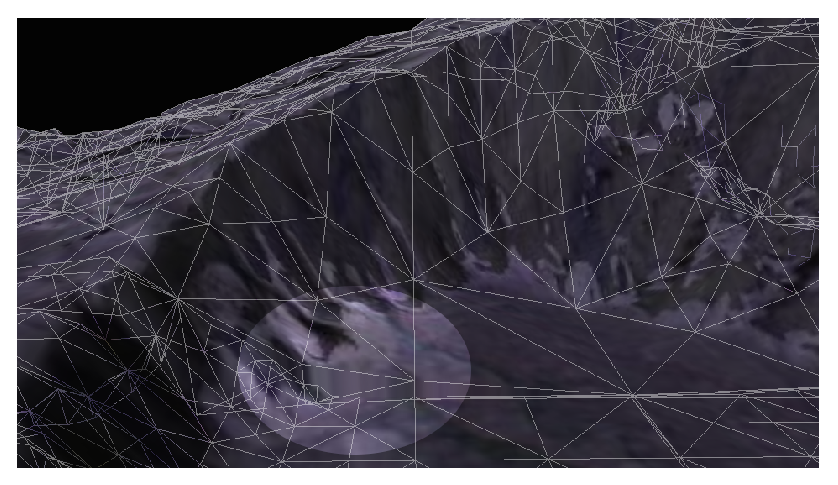
\includegraphics[width=6in]{sig-fig-stretch}
\caption{ Texture stretching on vertical skirt (in highlighted area).
$\tau$ has been set to 35 to illustrate stretching.  For more
normal values of $\tau$ (usually $< 5$), texture stretch is very
hard to see. }
\label{fig:stretch}
\end{figure}

\section{Avoiding Pops}

As mentioned above, we can hide the ugly visual transition when a
chunk splits into it s child chunks, or when child chunks merge into a
parent chunk.  The solution involves applying a small (possibly 0)
morph to the vertical coordinate of each vertex in a chunk mesh, using
a single uniform morph parameter over the whole chunk.  The morph
target is computed as follows: for each vertex in a chunk, its morph
target has the same horizontal coordinates.  The vertical coordinate
is computed by sampling the height of the parent chunk and the known
horizontal coordinates.
 
At rendering time, we will compute a chunk's morph parameter, ensuring
that the morph parameter is always 0 when the chunk is about to split,
and 1 when the chunk is about to merge.  This guarantees that the
shape of a chunk at the distance where a split occurs is identical to
the shape of the chunk chunks at an infinitesimally closer distance,
after the chunk has split.


\begin{figure}[h]
\includegraphics[width=6in]{sig-fig-pop-avoid}
\caption{A 2D illustration of pop avoidance.  On the left is a line
with two vertices, representing part of a low-detail chunk.  In the
middle, it has been replaced by a line with three vertices,
representing a higher detail child chunk.  The dashed line shows the
desired true shape of the chunk, but the middle vertex has been
morphed to match the low-detail parent chunk.  On the right, the
middle vertex has morphed into its desired position.}
\label{fig:pop-avoid}
\end{figure}

Rearranging our error metric, we can directly compute such a morph
parameter given the distance to the chunk.

\begin{equation}
t_{morph} = clamp(\frac{ 2 \rho }{ \tau } - 1, 0, 1)
\label{eqtmorph}
\end{equation}
 
This formula produces $t_{morph} = 0$ at the distance at which the
chunk's parent splits (because the parent's $\delta$ is double the
child's $\delta$, and the parent's bounding volume contains the child).
It produces $t_{morph} = 1$ exactly at the point at which the chunk
itself will split.  It linearly interpolates $t_{morph}$ in between
those distances, as the viewer gets close to the chunk.
 
This avoids the visual artifact caused by many simultaneous vertex
pops.  In fact, it completely eliminates all vertex pops throughout
the tree, replacing them instead with a subtle morph.  The actual LOD
transition when a chunk is split into its children is completely
undetectable to the viewer.  Note that when using our simple error
metric, morphing is based entirely on viewpoint distance, which has
the nice property that the mesh only morphs when the viewpoint moves.
This further reduces the noticeability of morphing.
 
The data cost of this morphing scheme is the addition of either a
morph target or a morph delta per vertex.  A morph delta may be
preferred because it can be quantized into very few bits.  The morph
delta will always be smaller than $\tau$ pixels on-screen, so the
quantization error in screen space is less than $\tau / (2^N)$
where $N$ is the number of bits allocated for the morph delta.
 
There is also the on-the-fly processing required to adjust the vertex
data.  Because the morph parameter is uniform over an entire chunk,
and the vertex data for a chunk is just a simple linear array, even a
naive CPU implementation is fast enough to feed a hungry GPU pipeline.
For reduced CPU load, a straightforward vertex program (vertex shader)
may be used instead.
 
\section{Texturing}

Texturing for this LOD scheme is very simple --- at preprocessing time,
we just provide a static texture for each static chunk.  Given
knowledge of the screen-space error metric used at run-time, and an
upper bound on the runtime value of $\tau$, our preprocessor can
guarantee that the projected texel size at run time will not exceed 1
texel per pixel.  The math goes like this: Let $D_{min}$ be the
minimum geometric distance at which a chunk will be displayed.  From
formula 1, we have:
 
\begin{equation}
D_{min} = \frac{ \delta }{ \tau } K
\end{equation}
 
and also,
 
\begin{equation}
T_s \leq \frac{ T_g }{ D_{min} } K
\end{equation}
 
where $T_s$ is the projected size of a texel on-screen, and $T_g$ is
the geometric size of a texel for the texture of a chunk.  Solving for
$T_g$, and substituting 1 for $T_s$ we get:
 
\begin{equation}
T_g \leq \frac{ \delta }{ \tau }
\end{equation}
 
We can use this formula for $T_g$ to force a minimum texture
resolution for each chunk at preprocessing time.  Note that if we are
using a simple 2D mapping to assign texture coordinates, this formula
does not account for texture stretch due to steeply sloping surfaces.
We can optionally compute texture stretch as well, based on the known
chunk geometry, and take it into account.
 
\section{Compression}

The chunk hierarchy, crack-filling meshes, and vertex morphing
information impose a substantial size overhead on the storage required
for a chunk tree, compared to a simple static mesh of the same object
or a heightfield representation.  However, there are a couple of
significant factors which help offset this overhead.
 
The preprocessing step in Chunked LOD completely discards vertices
which are not necessary to approximate the mesh to within the minimum
value of $\delta$ (at the highest LOD in the tree).  This acts as a form
of lossy compression on the original heightfield.  Flat areas are
heavily decimated.  For typical real-world DEM models, the compression
is usually significant, even for very modest degradation in the
heightfield shape.
 
Another potentially useful property of Chunked LOD is that the
vertices in individual chunks are spatially localized.  The chunks
vary in size in world coordinates, but because of the LOD algorithm,
stay within restricted bounds in screen coordinates.  If the vertices
in a chunk are compressed using a simple quantization scheme, the
quantization errors will be bounded in screen space.  This fails to
hold true when zooming in on the finest chunk level; however, for
reasonable tree depths (e.g. up to 8 levels) 8 bits of precision
should be enough for even large data sets.
 
% table here?

Taking into account all overhead, the reference implementation of the
chunk preprocessor produces chunk data files (geometry only, no
textures) ranging from around 25 to 35 bytes per unique output vertex,
depending on the data and the preprocessing parameters.  For typical
DEM data and very modest lossy compression, this may correspond to
around 5 to 7 bytes per heightfield sample in the input data.  These
figures do not yet reflect the aggressive quantization compression
possibilities mentioned above, so a realistic minimum data size for
Chunked LOD will be smaller.
 
\section{Paging out-of-core chunks}

All mesh and texture data for each chunk is self-contained.  This
makes it fairly easy to page in detail on demand.  The general
approach is to run a separate thread which is responsible for loading
chunk data.  The render pseudocode is modified as follows:

\begin{ttfamily}
\begin{tabbing}
\hspace{0.25in}\=\hspace{0.25in}\=\hspace{0.25in}\=\hspace{0.25in}\=\hspace{0.25in}\= \\
function render\_lod(node)                                                      \\
\>      node.last\_used\_frame = current\_frame                                 \\
\>      if                                                                      \\
\>\>            not\_all\_child\_data\_resident(node)                           \\
\>      or                                                                      \\
\>\>            rho(node, viewpoint) $<=$ tau                   \\
\>      then                                                                    \\
\>\>            -- compute morph\_parameter                                     \\
\>\>            draw(node.geometry, morph\_parameter)                           \\
\>\>            for c in node.children do                                       \\
\>\>\>                  request\_residency(c)                                   \\
\>\>            end                                                             \\
\>      else                                                                    \\
\>\>            for c in node.children do                                       \\
\>\>\>                  render\_lod(c)                                          \\
\>\>            end                                                             \\
\>      end                                                                     \\
end
\end{tabbing}
\end{ttfamily}
 
Additionally the loading thread should free the storage used by a
node's geometry data when it has not been used for some time.
 
\section{Implementation}

% update vs render

% quadtree tiling, jpeg compression

% timings & results

I have made a free, public domain reference implementation of the
Chunked LOD algorithm presented here.  It runs on Windows and Linux,
and should be adaptable to other platforms.  I encourage anyone who is
interested to use and adapt the code for any purpose.  Credit, bug
fixes and improvements are always appreciated, of course, but there
are no restrictions whatsoever on how the code may be
used.\footnote{The code is available online at
http://sourceforge.net/projects/tu-testbed and is also linked from my
website at http://tulrich.com/geekstuff.}
 
\section{Acknowledgments}

Thanks are due to Oddworld Inhabitants for supporting the presentation
of this work and fostering a work environment where personal research
is encouraged.  Sean Barrett, Charles Bloom, Jon Blow, Mark
Duchaineau, Tom Forsyth, Josh Levenberg and Aaron Pfeiffer for
comments, criticism and ideas.  Thierry Berger-Perrin and Mike Shaver
for providing additional code, bug fixes, and Linux build
improvements.  John Ratcliff, Peter Lindstrom, Ben Discoe, Ken
Musgrave, the University of Washington and the US Geological Survey
for providing sample data.
 
\bibliographystyle{plain}
\bibliography{sig-notes}

\end{document}
